\section{Appendix}
\subsection{Data Collection: Technical Aspects \& Tools used}
\label{sec:appendix-data-collection}
The data-collection process was implemented in \emph{Python v3.9.12}. All implementations for the architectures such as VGG11 or individual layers such as the Convolution were taken from the \emph{PyTorch v1.11.0} framework with \emph{torchvision v0.12.0}. Furthermore, the package \emph{ptflops v0.6.9}\footnote{\url{https://github.com/sovrasov/flops-counter.pytorch}} was used to compute MAC counts, except for the MaxPool2d layer (see App.~\ref{sec:appendix-macs-computation}. Finally, the tool \emph{codecarbon v2.1.3}\footnote{\url{https://github.com/mlco2/codecarbon}}  was used to measure the energy consumption of each model and layer configuration. codecarbon accesses the Intel RAPL interface to read out the energy consumption of the CPU during the execution of a program. On the hardware side, the same machine of a slurm cluster with an Intel(R) Xeon(R) CPU E5-2630 v4 @ 2.20GHz and 256GB of memory was used for the entire process. The data collection was performed solely on the CPU and no GPU was employed. This decision was based on the common practice of using CPUs to run models at inference, and as \citet{misnomer} stated that 80-90\% of machine learning workload is dedicated to inference processing rather than training.

To reduce the noise and errors introduced by codecarbon, we measured the energy consumption by tracking as many forward passes through a module, as possible within a 30-second window. We then normalized this measurement by the number of forward passes, resulting in an average energy estimate for a single forward pass. To obtain even more precise measurements, we repeated this process up to three times per configuration and took the average of the results. It should also be mentioned that on rare occasions codecarbon logged an error while measuring, but because we collected at least three data points per configuration, we were able to remove these erroneous observations, without losing information.
% --------------------------------------------------------
%
% --------------------------------------------------------
\subsection{Computer Performance Measures}
\label{sec:appendix-performance-measures}
The number of \emph{Floating Point Operations}, in short \emph{FLOPs}, is a performance measure in computing that is widely used to determine the capabilities of a computer. The metric is defined as the total number of basic machine operations (floating-point additions or multiplications) that need to be executed by a program. Floating point operations often have a higher latency than other types of operations, which can greatly impact a program's overall execution time. This makes them a useful proxy for determining said execution time \citep{Dissecting_DBLP:journals/corr/abs-2107-11949}.

In this work, we are interested in the number of FLOPs that are required to compute a single forward pass through a deep CNN such as VGG11, as well as for all the individual layers/operations in the architecture. In deep learning, the type of operation that often dominates the number of FLOPs is the matrix-matrix product. Thus, the deeper the architecture, the more matrix-matrix products need to be computed, which results in a proportional increase in the number of FLOPs \citep{Dissecting_DBLP:journals/corr/abs-2107-11949}. Since the number of FLOPs can be seen as a proxy to the model's execution time, it can also be seen as a proxy for the energy consumption of the same model (on the given hardware)\citep{Energy-based_DBLP:journals/corr/abs-1808-00286}. Another popular and very similar metric is the MAC count (multiply-accumulate operations), which is better suited to represent operations such as matrix-matrix products. A single MAC is defined as the product of two numbers where the result of said product is then added to an accumulator. Modern systems are often capable of computing a MAC as a single operation, thus making the computation of matrix-matrix products more efficient. An approximate translation from FLOPs to MACs can be achieved by simply dividing the number of FLOPs by two. Because matrix-matrix products are incredibly important to the domain of deep learning and, as already mentioned, dominate the computational complexity of current models, we only refer to the MAC count in this work and translate from FLOPs to MACs where necessary.
\subsubsection{Computation of MAC count for each layer type}
\label{sec:appendix-macs-computation}
In the following, the computation of the number of MACs required for a forward pass through a variety of layer types will be discussed. Generally, the number of MACs for a CNN such as VGG11 is computed as the sum of layer-wise MAC counts. Given that the Convolution is an important layer of any CNN architecture, we will begin by introducing the MACs formula for this layer type. Note the following terminology: the input/output width of a Convolution will be referred to by $w_{in}/w_{out}$ and the input/output height by $h_{in}/h_{out}$. Accordingly, the number of input/output channels will be given by $c_{in}/c_{out}$. Furthermore, $k$ will correspond to the size of a symmetric kernel, $P$ to the padding parameter, and $B$ to the batch-size. Given this, the MAC count for a single forward pass through a Convolutional layer is given by:
$$\#MACs(Convolution) = k^2 * w_{out} * h_{out} * c_{in} * c_{out} * B$$
Tab.~\ref{tab:mac-count-formulas} shows the formulas for all other relevant components and layer types mentioned in this work. Note that both the ReLU activation and the MaxPooling layer do not require any multiply-accumulate operations, which is why we divide the number of FLOPs by two to approximate the MAC count.
\begin{table}[t]
    \caption{MAC count formulas for all relevant components and functions required in paper; the third column gives sum of the MACs for all instances of the given layer type for a single forward pass through VGG11 with $B=1$.}
    \label{tab:mac-count-formulas}
    \begin{center}
        \begin{tabular}{l|lllll}
        \multicolumn{1}{l}{\bf Module}  & \multicolumn{1}{l}{\bf MAC Formula} & \multicolumn{1}{l}{\bf VGG11 Example}
\\ \hline \\
\textbf{Convolution}    & $k^2 * w_{out} * h_{out} * c_{in} * c_{out} * B$      & 7492882432 \\
\textbf{Linear}& $w_{in} * h_{in} * c_{in} * c_{out} * B$              & 123642856 \\
\textbf{MaxPooling}     & ($k^2 * w_{out} * h_{out} * c_{in} * B)/2$            & 3060736 \\
\textbf{ReLU}           & $(w_{in} * h_{in} * c_{in} * B)/2$                    & 3717120 \\
\end{tabular}
    \end{center}
\end{table}
% --------------------------------------------------------
%
% --------------------------------------------------------
\subsection{Adding real layer configurations to the training sets}
\label{section:add-real-configs}
The results presented in Sec.~\ref{sec:results} showed that the models for the Convolution and MaxPooling layers were struggling to generalize to configurations from real architectures. One hypothesis was that the random configurations used in the training sets may not be adequate representations of the layers in real-world architectures. This could be because the large number of parameters in these layers leads to a wide range of potential random configurations that are very unlikely to appear in any carefully conceptualize architecture. Thus, in the following experiment, we additionally measured the energy consumption of each individual configuration of Linear, Convolution, and MaxPooling layers present in AlexNet and VGG11/13/16 with a random batch-size and added these measurements to the training sets. After retraining, all models showed slight performance improvements when evaluated on the same task as in Sec.~\ref{sec:results}, resulting in an overall $R^2$ score of 0.45 (previously 0.352). The exact performance improvements for each layer can be seen in Tab.~\ref{tab:improvements-from-real-configs}. These results indicate that enriching the training set with \emph{individual} configurations similar to the ones present in larger models can improve the energy predictions on the \emph{full} models.

\begin{table*}[h]
    \caption{$R^2$ score performance improvements on layers present in \emph{full} architectures after adding measurements from \emph{individual} of the Convolution, MaxPooling, and Linear layer configurations present in the full architectures to the training data sets  models.}
    \label{tab:improvements-from-real-configs}
    \centering
    \begin{tabular}{l|ll}
        \multicolumn{1}{l}{\bf Module}  & \multicolumn{1}{l}{\bf score before}  & \multicolumn{1}{c}{\bf score after}
        \\ \hline \\
        \textbf{MaxPool2d} & 0.559 & 0.679 (+ 0.120) \\
        \textbf{Conv2d} & 0.314  & 0.395 (+ 0.081)\\
        \textbf{Linear} & 0.977 & 0.978 (+ 0.001) \\
    \end{tabular}
\end{table*}
\subsection{Predictive capabilities of various feature sets}
\label{sec:appendix-feature-sets-experiment}
To find the best possible model for each layer type, we experimented with a variety of different feature combinations, and a separate model was fitted and fine-tuned to each, trying to maximize the performance in that setting. Thus, in the following, we will refer to the \emph{parameter-set} as a feature set that only contains the standard layer parameters, the \emph{(log+)parameter-set}, which in addition to the standard layer parameters also contains the log-transformed parameters, the \emph{parameter-MAC-set} as the feature set that contains both the layer parameters and the MAC count as features and finally the \emph{(log+)parameter-MAC-set} which contains all of the previously mentioned features. Additionally, we attempted to model each layer with the MAC count as the only feature. For all feature sets that contain the MAC count, we applied a StandardScaler before fitting the model to compensate for the large differences in magnitude between the parameters and the MAC count. The goal of this experiment was to analyze which feature combination would have the best predictive qualities for each layer. This analysis was not conducted for the activation functions.  For more details on the performance of all models, features-sets, and layer types please see Tab.~\ref{tab:feature-set-performances}.

\textbf{Linear layer}. All models are Linear regressors with the parameter- and (log+)parameters-set models having additional interaction-only polynomial features of degree $d=3$. Each one of the five configurations achieved an outstanding $R^2$ score of at least 0.999, with the model based on the parameter-set scoring the lowest ($R^2$ 0.999). To help with feature selection, a Lasso regressor was also used with the (log+)parameters-set, but showed no improvements over a standard Linear regressor. 

\textbf{Convolutional layer}. The models based on the parameter- and (log+)parameter-sets were Lasso regressors with additional interaction-only polynomials of $d=3$ and $d=4$. Even though the Lasso models proved to be slightly more robust than standard Linear regressors, the models performed poorly with the former achieving an $R^2$ score of 0.7097 and the latter only performing slightly better with a score of 0.7954. The MAC-count-only Linear regressor showed a significant boost in performance with an $R^2$ score of 0.9977. Further small improvements could be achieved by combining the (log+)parameter-sets with the MAC count in a Linear regressor for a $R^2$ score of 0.9979. Sec.~\ref{sec:appendix-ablation-analysis} of the Appendix gives further insights on feature importances through an ablation analysis. 

\textbf{MaxPooling layer}. Similar to before, we trained two Lasso regressors based on the parameter- and (log+)parameter-sets, with additional interaction-only polynomial features of $d=4$ and $d=3$. While the former performed poorly with an $R^2$ score of only 0.4468, the latter with log-features performed significantly better with an $R^2$ score of 0.8194. Even though further increasing the degree of the polynomials resulted in slightly better scores, the models were less robust. In accordance with previous results, the feature sets, which contained the MAC count caused a significant uplift in performance, with the (log+)parameter-MAC- and parameter-MAC-set performing almost identically with a $R^2$ score of $0.9995$ and $0.9967$. The MAC count only model performed the worst of the three with an $R^2$ score of $0.9797$.

The goal of this experiment was to analyze the predictive capabilities of the various feature sets for the different layer types. Each model for each layer-feature-set combination was carefully fitted and evaluated to achieve the best possible performance. The experiment has shown that A) the MAC count feature is vital when it comes to predicting the energy consumption and may even be sufficient to do so, B) polynomial features are helpful when modeling energy consumption, and C) while Lasso regressors can help with feature selection, they do not provide significant improvements in these experiments.
% --------------------------------------------------------
%
% --------------------------------------------------------
\subsection{Ablation analysis: Convolutional Layer}
\label{sec:appendix-ablation-analysis}
In the following experiment, we conducted an ablation analysis with the Convolutional layer model. The model is based on the (log+)parameter-MAC-set, which contains all the possible features for this layer (see App.~\ref{sec:appendix-feature-sets-experiment} for details). The model is a Linear regressor with a StandardScaler applied to the features before fitting. The experiment was conducted as follows. For each one of the 32767 possible feature subsets of minimum size one, we fitted the model and reported the test scores and errors. The goal of the experiment was to see, which features are the most important and which exact combination of features would lead to the best results. No polynomial features were included in this analysis as that would cause a combinatorial explosion.

The results once again show that the MAC count is a very important predictor for the model. The maximum $R^2$ score for all models without this feature is only 0.25, while with the MAC count the score jumps to 0.998. Not only is the $R^2$ score with this feature substantially higher than without it, but also independent of the other features the score never reaches below 0.997. Furthermore, we observe that there are only very small performance deviations within the models that contain the MAC count. For all other feature sets, we observe much stronger changes in performance. Fig.~\ref{fig:ablation-analysis} illustrates this behavior and shows the performance of each feature set with and without the MAC count. Tab.~\ref{tab:ablation-analysis-results} shows the best and worst feature sets for both categories.
\begin{table*}[ht]
    \caption{Shows the best and worst feature combinations with their $R^2$ scores for both categories.}
    \label{tab:ablation-analysis-results}
    \centering
    \resizebox{1 \textwidth}{!}{
    \begin{tabular}{p{0.15\linewidth} p{0.42\linewidth} | p{0.42\linewidth}}
        \multicolumn{1}{c}{\bf Score}  & \multicolumn{1}{c}{\bf with MAC}  & \multicolumn{1}{c}{\bf without MAC}
        \\ \hline \\
        \textbf{highest score} & batch-size, image-size, kernel-size, in-channels, stride, log-image-size, log-kernel-size, log-out-channels, log-stride, log-padding, macs ($R^2$ $0.998$) & batch-size, image-size, kernel-size, in-channels, stride, log-batch-size, log-image-size, log-kernel-size, log-out-channels, log-stride ($R^2$ $0.25$) \\
        \\ \hline \\
        \textbf{lowest score}  & out-channels, log-out-channels, macs ($R^2$ $0.997$) & padding, log-padding ($R^2$ $-0.026$)\\
    \end{tabular}
    }
\end{table*}
% --------------------------------------------------------
%
% --------------------------------------------------------
\subsection{Additional Tables}
\begin{table}[h]
\caption{Shows the performance metrics for each layer type and feature set; the \emph{ito} in the \emph{Polynomial} column specifies that the polynomial features were restricted to interaction-only terms; the feature sets marked with a * were selected for the computation of the final estimates presented in Sec.~\ref{sec:results}}
\label{tab:feature-set-performances}
    \centering
    \resizebox{1 \textwidth}{!}{
    \begin{tabular}{lllcccccc}
            \multicolumn{1}{c}{\bf Module}  & \multicolumn{1}{c}{\bf Feature-Set}  & \multicolumn{1}{c}{\bf Polynomial} & \multicolumn{1}{c}{\bf StandardScaler} & \multicolumn{1}{c}{\bf Model} & \multicolumn{1}{c}{\bf Avg. $R^2$ Cross-Val} & \multicolumn{1}{c}{\bf Avg. MSE Cross-Val} & \multicolumn{1}{c}{\bf $R^2$ Test Set} & \multicolumn{1}{c}{\bf MSE Test-Set}
            \\ \hline \\
            \textbf{Conv2d}     & parameter             & d=4, ito & n & Lasso & 0.513 (± 0.293) & -2.467e-03 (± 1.889e-03) & 0.7097 & 3.490e-03  \\
                                & (log+)parameter       & d=3, ito & n & Lasso & 0.622 (± 0.192) & -2.105e-03 (± 1.734e-03) & 0.7954 & 2.460e-03  \\
                                & MACs*                  & & n & Linear & 0.994 (± 0.005) & -2.291e-05 (± 1.329e-5) & 0.9977 & 2.779e-05  \\
                                & parameter-MAC        & & y & Linear & 0.996 (± 0.004) & -1.644e-05 (± 9.509e-06) & 0.9979 & 2.501e-05  \\
                                & (log+)parameter-MAC  & & y & Linear & 0.996 (± 0.004) & -1.560e-05 (± 9.004e-06) & 0.9979 & 2.578e-05  \\
            \textbf{MaxPool2d}  & parameter             & d=4, ito & n & Lasso & 0.528 (± 0.185) & -1.375e-03 (± 1.941e-03) & 0.4468 & 9.338e-04  \\
                                & (log+)parameter       & d=3, ito & n & Lasso & 0.704 (± 0.139) & -1.139e-03 (± 2.137e-03) & 0.8194 & 3.048e-04  \\
                                & MACs                  & & n & Linear & 0.946 (± 0.051) & -9.746e-05 (± 7.278e-05) & 0.9797 & 3.431e-05  \\
                                & parameter-MAC        & d=2, ito & y & Linear & 0.993 (± 0.005) & -3.043e-05 (± 5.706e-05) & 0.9967 & 5.533e-06  \\
                                & (log+)parameter-MAC*  & d=2, ito & y & Linear & 0.999 (± 0.000) & -2.552e-06 (± 4.612e-06) & 0.9995 & 7.736e-07  \\
            \textbf{Linear}     & parameter             & d=3, ito &n& Linear & 0.999 (± 0.000) & -3.784e-05 (± 1.300e-05) & 0.9990 & 3.848e-05  \\
                                & (log+)parameter       & d=3, ito &n& Linear & 0.999 (± 0.000) & -2.756e-05 (± 1.179e-05) & 0.9995 & 1.839e-05  \\
                                & MACs*                  &&n& Linear & 0.999 (± 0.000) & -4.284-05 (± 1.425e-05) & 0.9992 & 3.384e-05  \\
                                & parameter-MAC        &&y& Linear & 0.999 (± 0.000) & -3.909e-05 (± 1.313e-05) & 0.9991 & 3.693e-05  \\
                                & (log+)parameter-MAC  &&y& Linear & 0.999 (± 0.000) & -3.466e-05 (± 1.147e-05) & 0.9992 & 3.134e-05  \\
            \textbf{ReLU}       & parameter             & d=2, ito & n & Linear & 0.981 (± 0.004) & -1.040e-03 (± 2.158e-04) & 0.9812 & 8.991e-04  \\
                                & MACs*                 & & n & Linear & 0.981 (± 0.005) & -1.046e-03 (± 2.284e-04) & 0.9812 & 1.030e-03  \\
            \textbf{Sidmoid}       & parameter*             & d=2, ito & n & Linear & 0.981 (± 0.008) & -1.047e-03 (± 1.866e-04) & 0.9905 & 7.538e-04  \\
            \textbf{Tanh}       & parameter*             & d=2 & n & Linear & 0.976 (± 0.008) & -1.315e-03 (± 4.252e-04) & 0.9761 & 1.412e-03  \\
            \textbf{Softmax}       & parameter*             & d=2, ito & n & Linear & 0.989 (± 0.004) & -5.671e-04 (± 1.599e-04) & 0.9913 & 4.972e-04  \\
                                
    \end{tabular}
    }
\end{table}
\begin{table}[h]
    \caption{Shows the number of unique and total data points that were collected for each PyTorch module; for the architectures, the number of data points also includes the data points for all individual layers, for each measurement of the full architecture.}
    \label{tab:data-sets}
    \begin{center}
        \begin{tabular}{llllll}
        \multicolumn{1}{c}{\bf Module} & \multicolumn{1}{c}{\bf Number of unique data points/configurations}  & \multicolumn{1}{c}{\bf Total data points}
\\ \hline \\
\textbf{Conv2d}     & 976 & 2900 \\
\textbf{MaxPool2d}  & 985 & 2939 \\
\textbf{Linear}     & 992 & 2962 \\
\textbf{ReLU} & 988 & 2951 \\
\textbf{Sigmoid} & 489 & 1467 \\
\textbf{Softmax} & 493 & 1479 \\
\textbf{Tanh} & 491 & 1473 \\
\textbf{AlexNet, VGG11/13/16} & 1840 (including layers) &  5801 (including layers)\\
\end{tabular}
    \end{center}
\end{table}
% --------------------------------------------------------
%
% --------------------------------------------------------
\newpage
\subsection{Additional Figures}
\begin{figure}[h]
        \centering
        \begin{subfigure}[b]{0.47\textwidth}
            \centering
            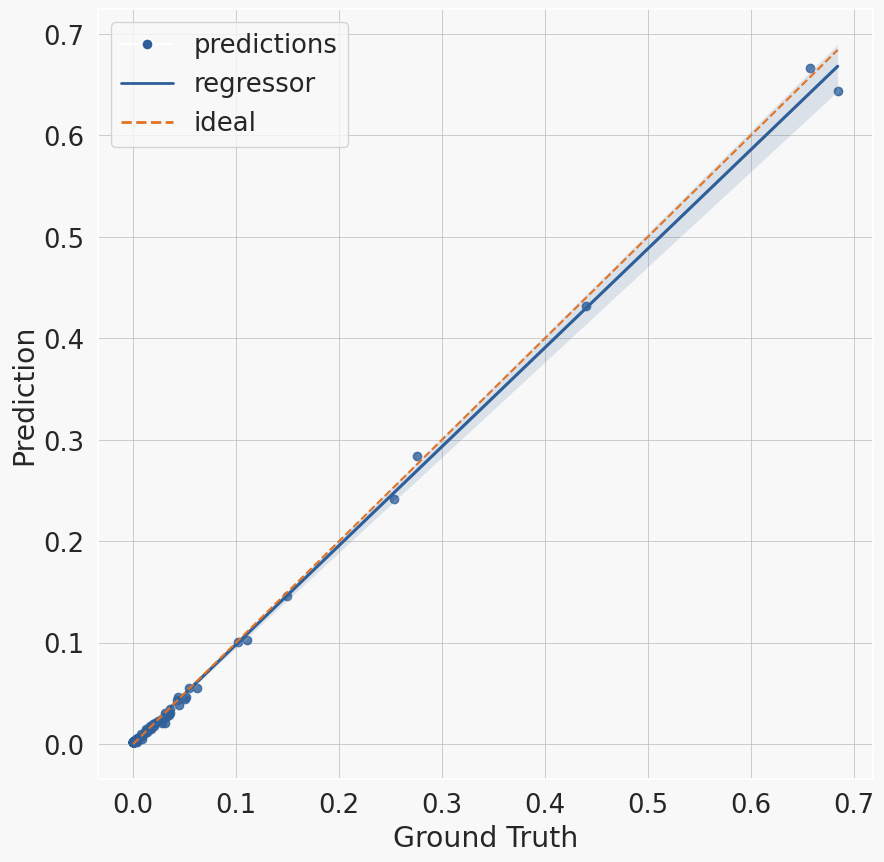
\includegraphics[width=\textwidth]{resources/scatter-conv.png}
            \caption[]%
            {{\small Convolution}}    
            \label{fig:layer-scatterplots convolution}
        \end{subfigure}
        \hfill
        \begin{subfigure}[b]{0.47\textwidth}  
            \centering 
            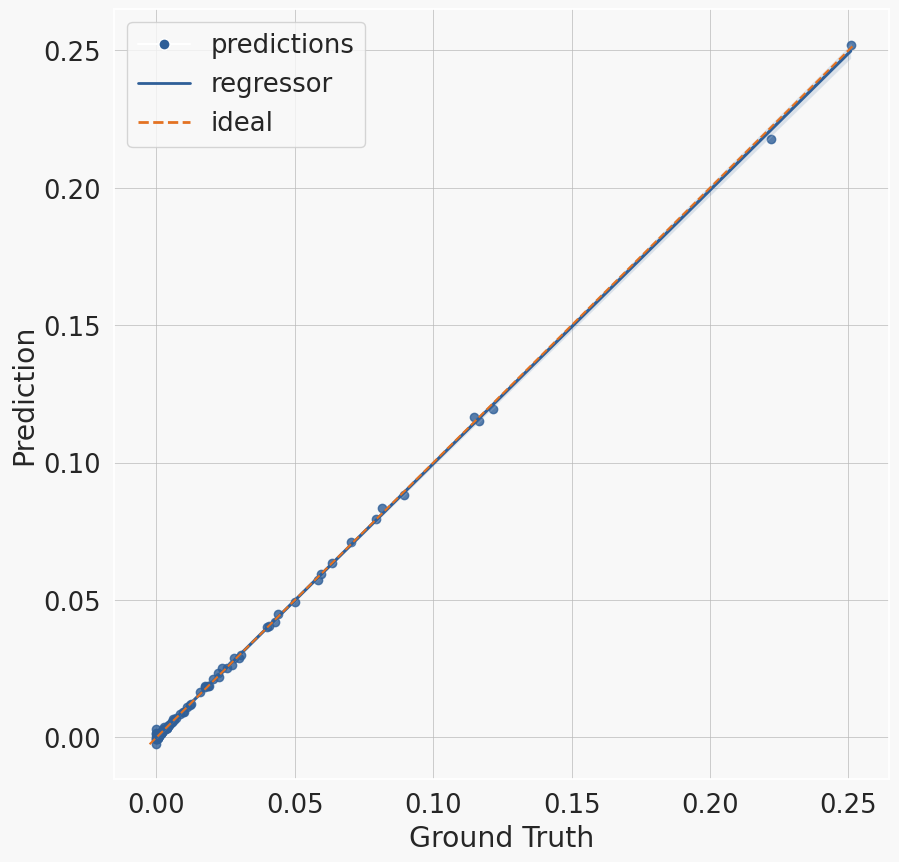
\includegraphics[width=\textwidth]{resources/scatter-maxpooling.png}
            \caption[]%
            {{\small MaxPooling}}    
            \label{fig:layer-scatterplots maxpooling}
        \end{subfigure}
        \begin{subfigure}[b]{0.47\textwidth}   
            \centering 
            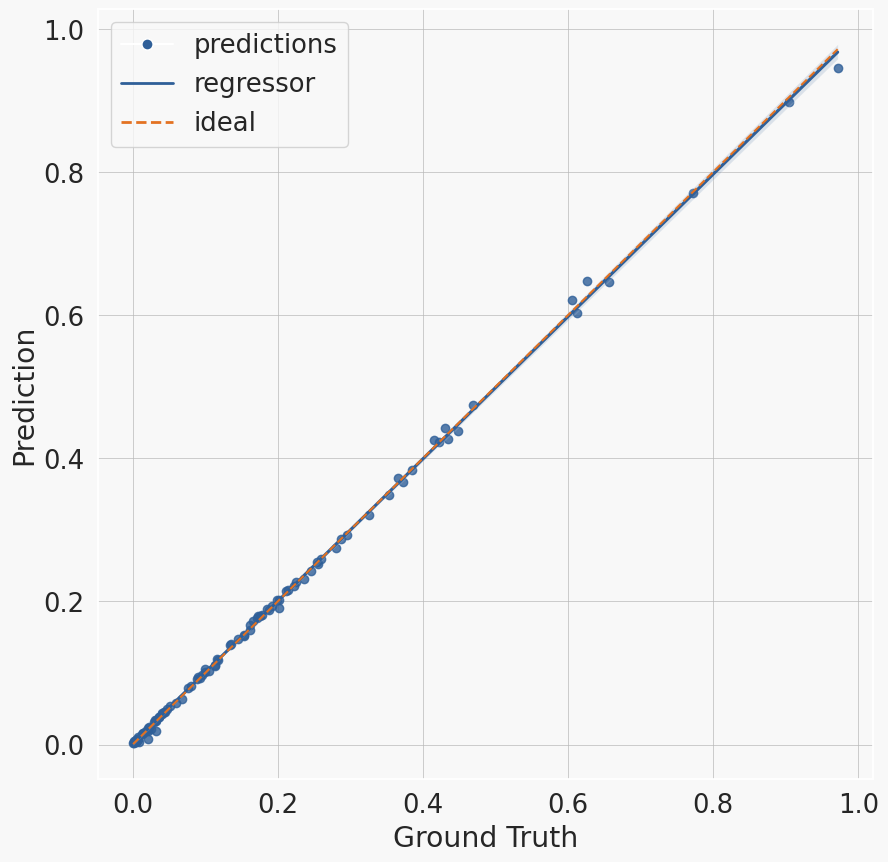
\includegraphics[width=\textwidth]{resources/scatter-linear.png}
            \caption[]%
            {{\small Linear}}    
            \label{fig:layer-scatterplots linear}
        \end{subfigure}
        \caption[Shows scatter-plots for the selected layer models (see Sec.~\ref{sec:results}), illustrating the accuracy of the predictions on the random test data; the x-axis represents the ground truth while the y-axis represents the predicted values, and the diagonal line symbolizes perfect predictions.]
        {Shows scatter-plots for the selected layer models (see Sec.~\ref{sec:results}), illustrating the accuracy of the predictions on the random test data; the x-axis represents the ground truth while the y-axis represents the predicted values, and the diagonal line symbolizes perfect predictions.}
        \label{fig:layer-scatterplots-layers}
\end{figure}
\begin{figure}[h]
        \centering
        \begin{subfigure}[b]{0.47\textwidth}
            \centering
            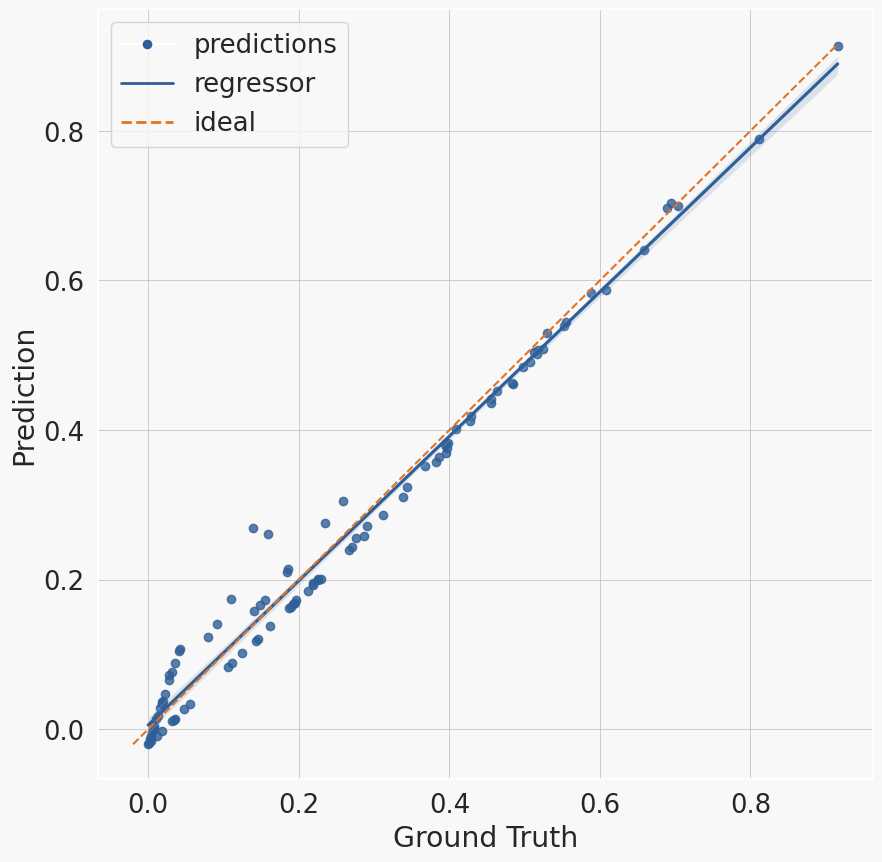
\includegraphics[width=\textwidth]{resources/scatter-relu.png}
            \caption[]%
            {{\small ReLU}}    
            \label{fig:layer-scatterplots relu}
        \end{subfigure}
        \hfill
        \begin{subfigure}[b]{0.47\textwidth}  
            \centering 
            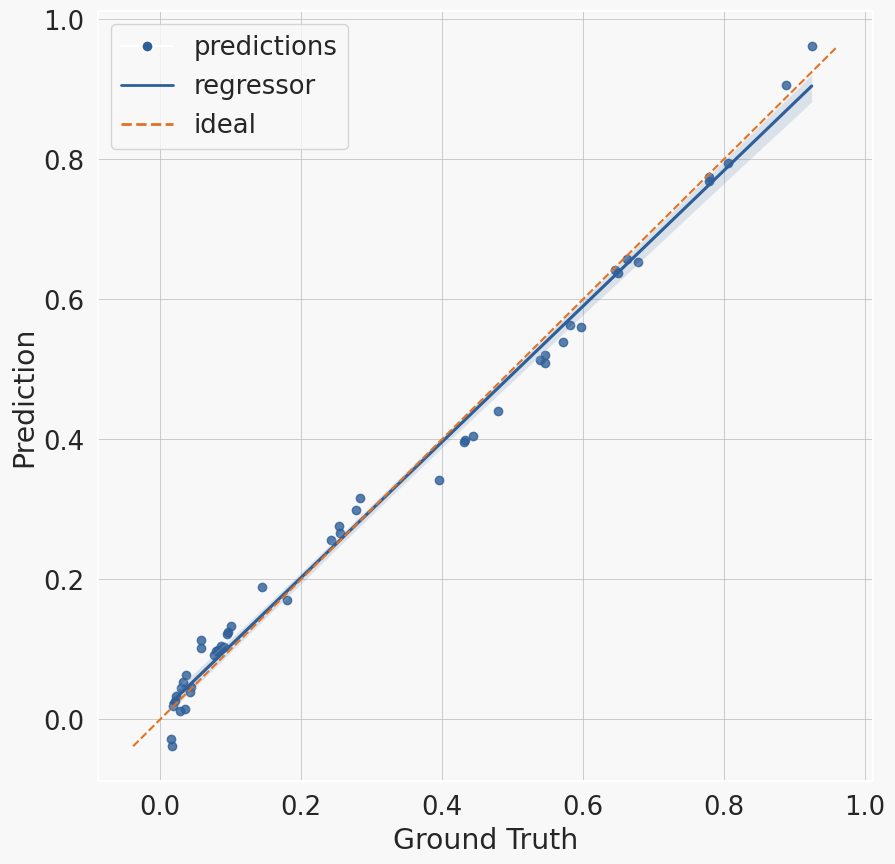
\includegraphics[width=\textwidth]{resources/scatter-sigmoid.png}
            \caption[]%
            {{\small Sigmoid}}    
            \label{fig:layer-scatterplots sigmoid}
        \end{subfigure}
        \vskip\baselineskip
        \begin{subfigure}[b]{0.47\textwidth}   
            \centering 
            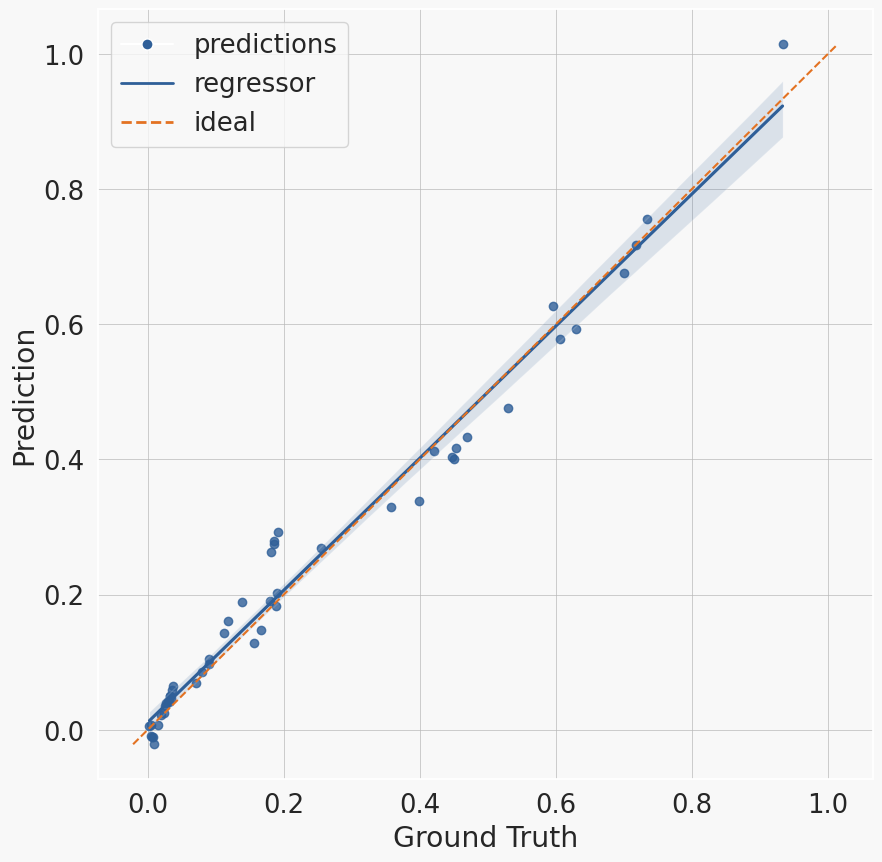
\includegraphics[width=\textwidth]{resources/scatter-tanh.png}
            \caption[]%
            {{\small Tanh}}    
            \label{fig:layer-scatterplots tanh}
        \end{subfigure}
        \hfill
        \begin{subfigure}[b]{0.47\textwidth}   
            \centering 
            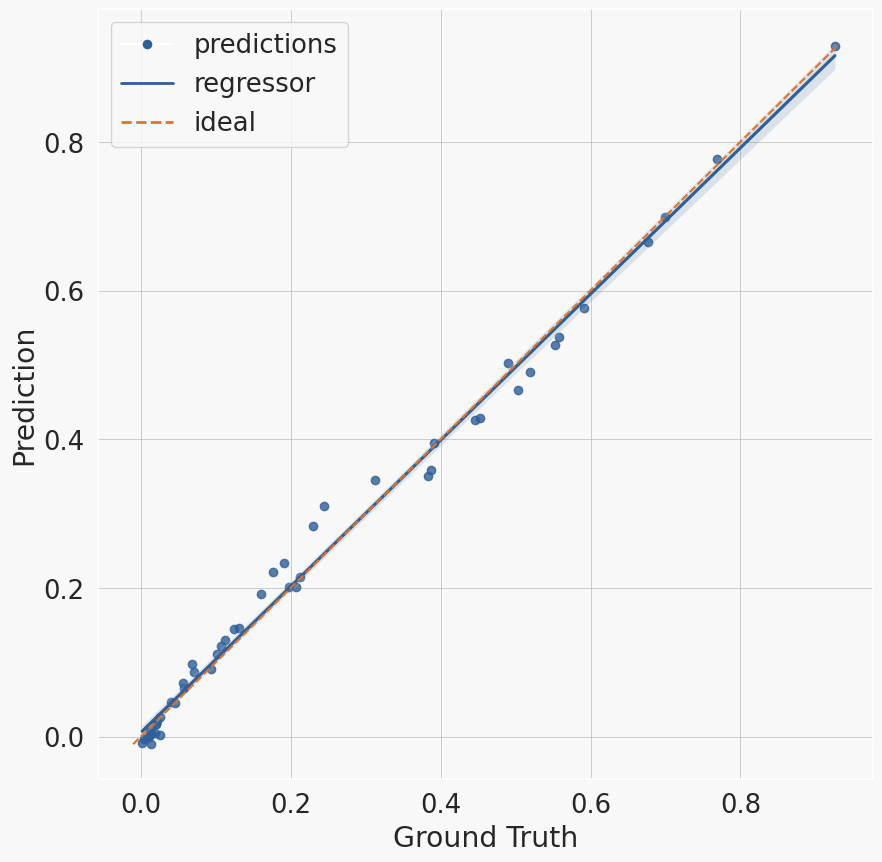
\includegraphics[width=\textwidth]{resources/scatter-softmax.png}
            \caption[]%
            {{\small Softmax}}    
            \label{fig:layer-scatterplots softmax}
        \end{subfigure}
        \caption[Shows scatter-plots for the selected activation models (see Sec.~\ref{sec:results}), illustrating the accuracy of the predictions on the random test data; the x-axis represents the ground truth while the y-axis represents the predicted values, and the diagonal line symbolizes perfect predictions.]
        {Shows scatter-plots for the selected activation models (see Sec.~\ref{sec:results}), illustrating the accuracy of the predictions on the random test data; the x-axis represents the ground truth while the y-axis represents the predicted values, and the diagonal line symbolizes perfect predictions.}
        \label{fig:layer-scatterplots-activations}
\end{figure}
\begin{figure}[h]
    \centering
    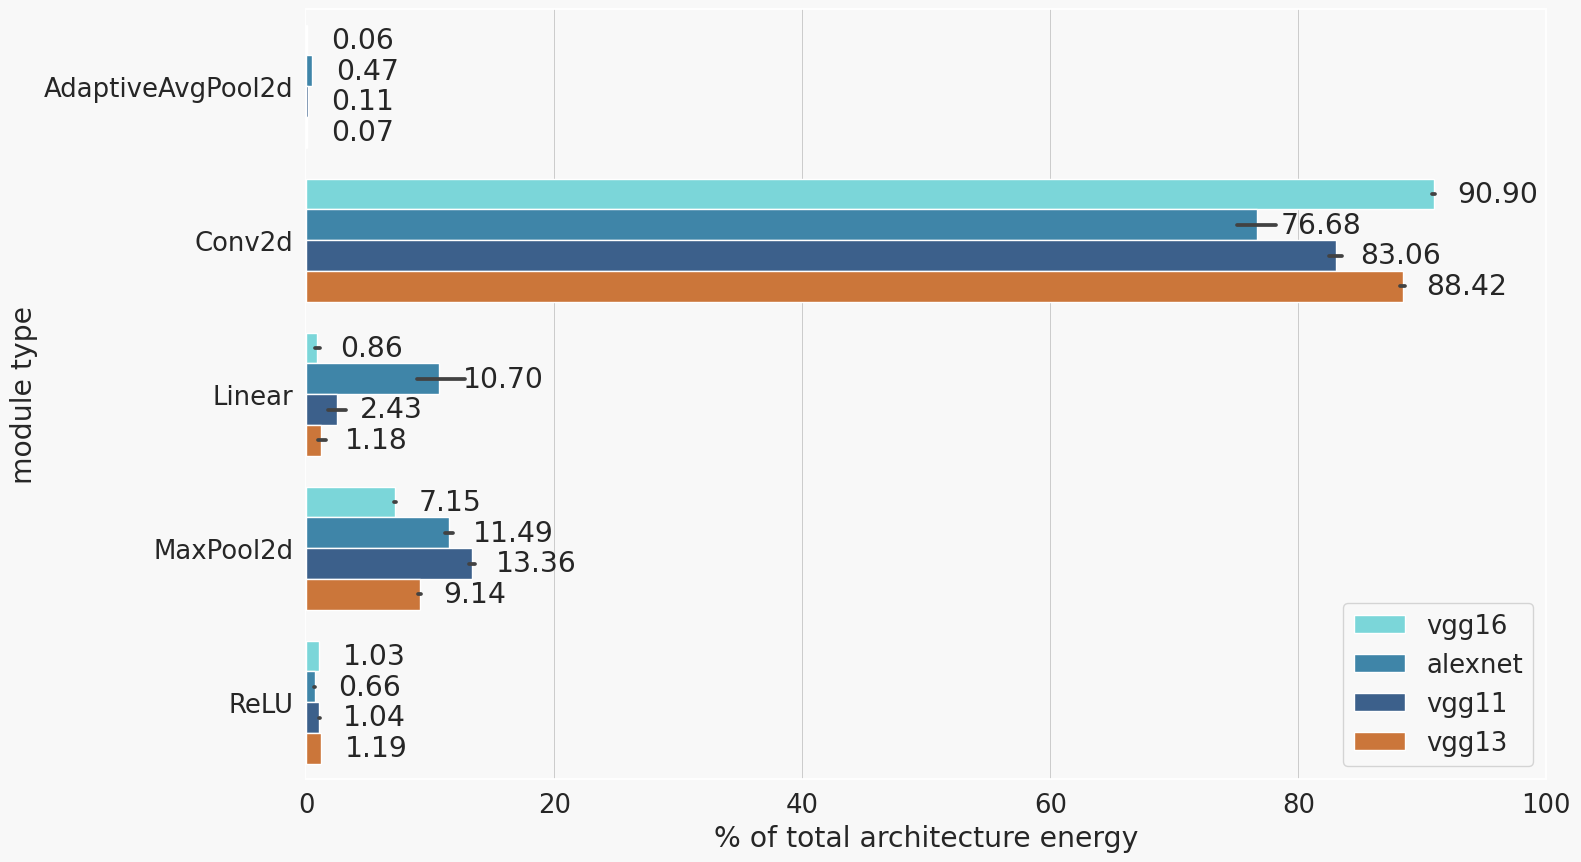
\includegraphics[width=0.9\textwidth]{resources/module-wise-energies.png}
    \caption{Shows the relative contributions of the individual layer types to the total energy consumption for AlexNet and VGG11/13/16; the black bars correspond to deviations caused by different batch sizes.}
    \label{fig:layer-wise-contribution}
\end{figure}
\begin{figure}
    \centering
    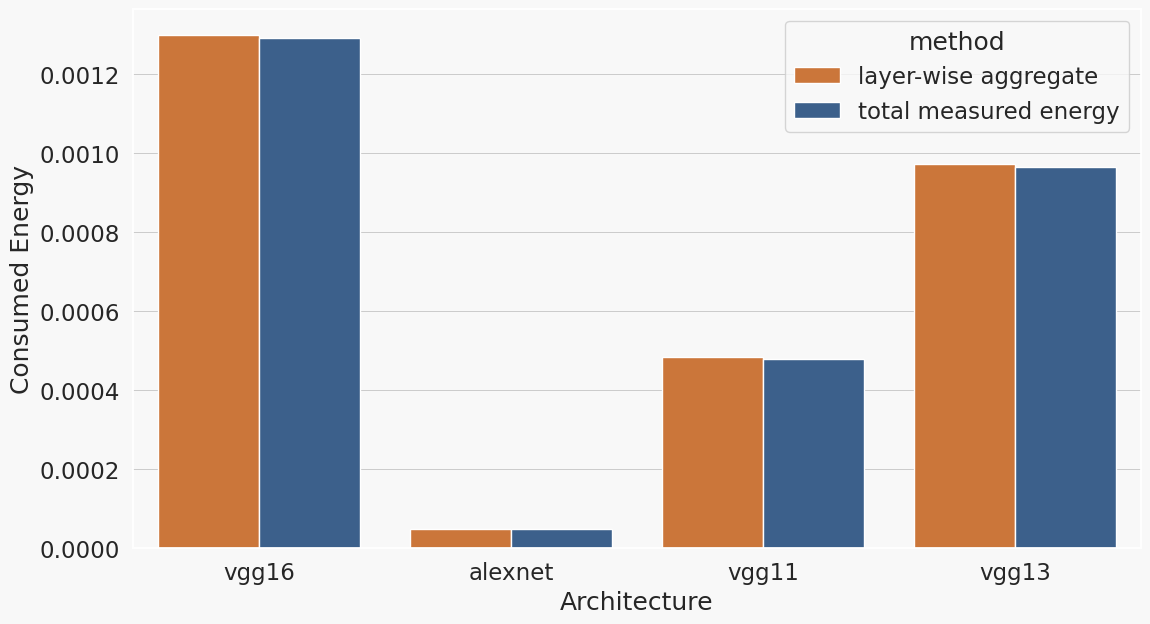
\includegraphics[width=0.9\textwidth]{resources/agg-vs-measured-energy.png}
    \caption{Compares the energy consumption of various architectures, when using two different measuring techniques; the ``total measured energy'' corresponds to the value obtained when measuring the architectures as singular units and the ``layer-wise aggregate'' corresponds to the sum of per layer measurements.}
    \label{fig:agg-vs-total-energy}
\end{figure}
\begin{figure}[t!]
    \centering
    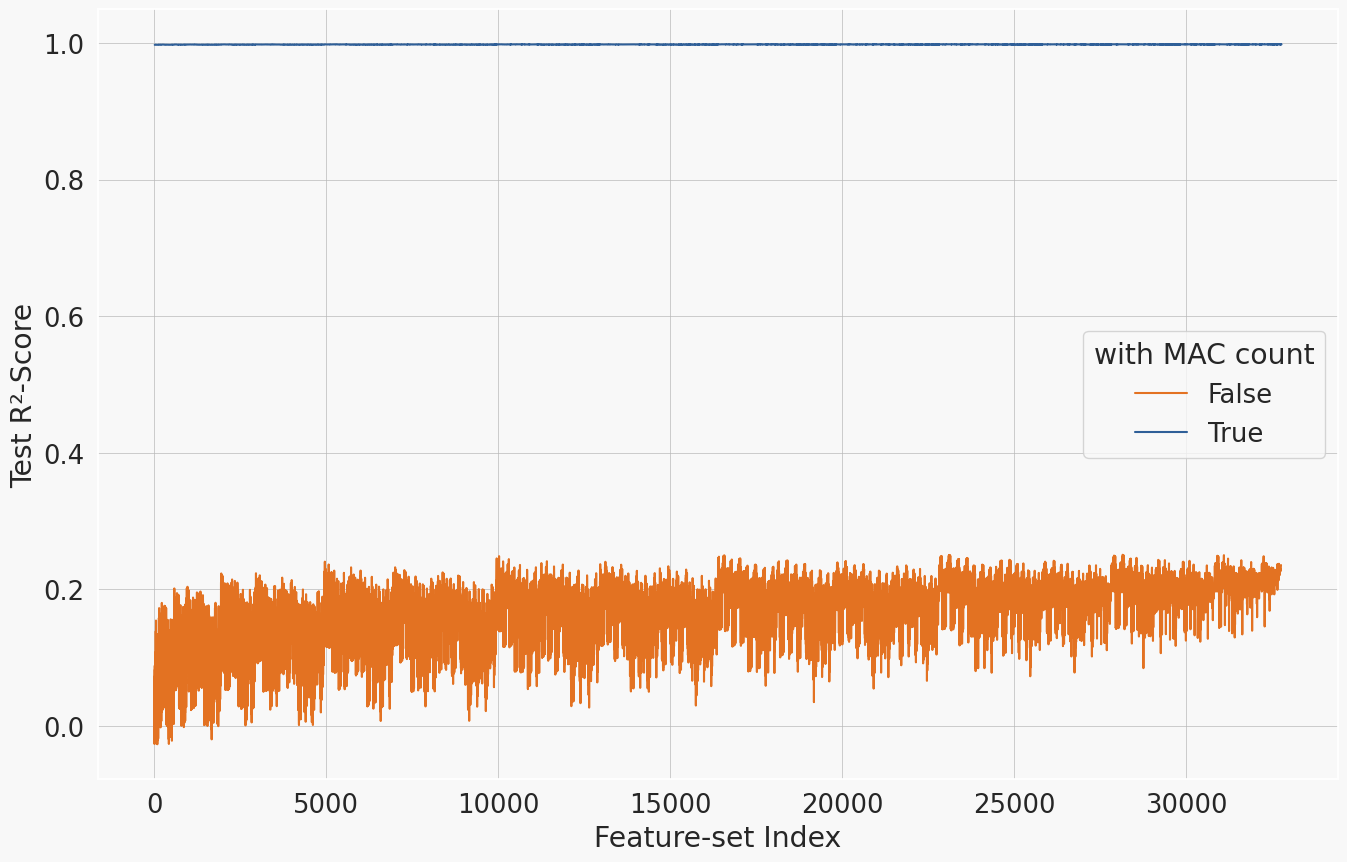
\includegraphics[width=0.9\textwidth]{resources/ablation-analysis.png}
    \caption{Shows the performance of all combinations of feature sets by their $R^2$ score; the x-axis corresponds to the feature set index and the y-axis to the $R^2$ score; the color indicates the whether the feature set contains the MAC count or not.}
    \label{fig:ablation-analysis}
\end{figure}